\begin{figure}
  \centering 
  \begin{subfigure}[b] 
{0.45\textwidth}
    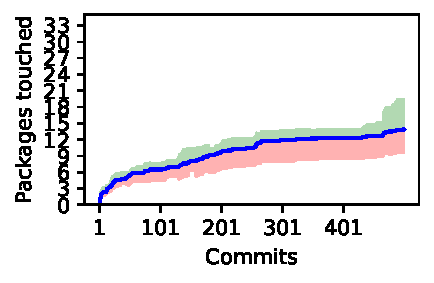
\includegraphics{sections/results/21/packages/time_series_components_touched.packages.all.founders.commits_500.pdf}
    \caption{Packages for All founders (n=10, $\mu$=14.1, median=9.0 \& std=6.22)}
    \label{figure.sections/results/21/packages/time_series_components_touched.packages.all.founders.commits_500.pdf}
  \end{subfigure}
  \begin{subfigure}[b] 
{0.45\textwidth}
    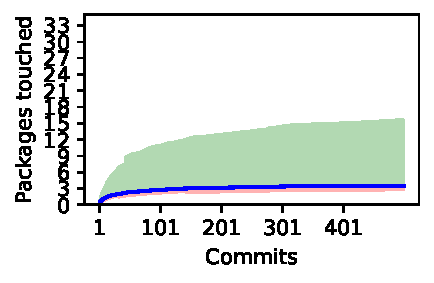
\includegraphics{sections/results/21/packages/time_series_components_touched.packages.all.joiners.commits_500.pdf}
    \caption{Packages for All joiners (n=521, $\mu$=5.5, median=1.0 \& std=8.8)}
    \label{figure.sections/results/21/packages/time_series_components_touched.packages.all.joiners.commits_500.pdf}
  \end{subfigure}
\newpage 
  \begin{subfigure}[b] 
{0.45\textwidth}
    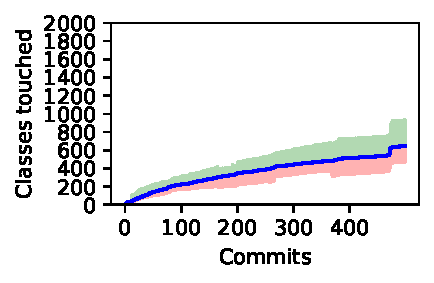
\includegraphics{sections/results/21/classes/time_series_components_touched.classes.all.founders.commits_500.pdf}
    \caption{Classes for All founders (n=10, $\mu$=644.7, median=296.0 \& std=328.93)}
    \label{figure.sections/results/21/classes/time_series_components_touched.classes.all.founders.commits_500.pdf}
  \end{subfigure}
  \begin{subfigure}[b] 
{0.45\textwidth}
    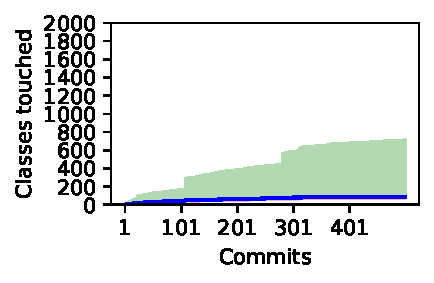
\includegraphics{sections/results/21/classes/time_series_components_touched.classes.all.joiners.commits_500.pdf}
    \caption{Classes for All joiners (n=521, $\mu$=90.51, median=4.0 \& std=225.57)}
    \label{figure.sections/results/21/classes/time_series_components_touched.classes.all.joiners.commits_500.pdf}
  \end{subfigure}
\newpage 
  \begin{subfigure}[b] 
{0.45\textwidth}
    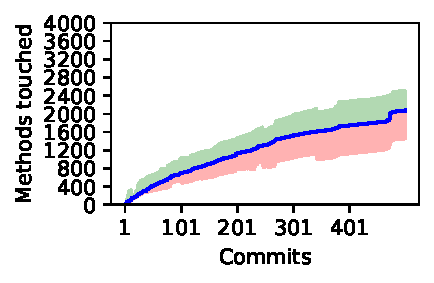
\includegraphics{sections/results/21/methods/time_series_components_touched.methods.all.founders.commits_500.pdf}
    \caption{Methods for All founders (n=10, $\mu$=2073.0, median=1010.0 \& std=1033.76)}
    \label{figure.sections/results/21/methods/time_series_components_touched.methods.all.founders.commits_500.pdf}
  \end{subfigure}
  \begin{subfigure}[b] 
{0.45\textwidth}
    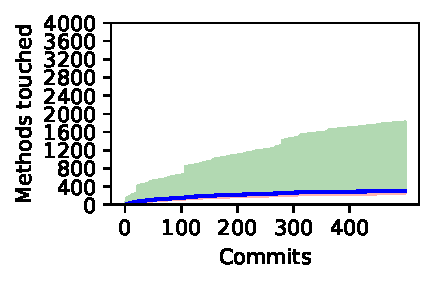
\includegraphics{sections/results/21/methods/time_series_components_touched.methods.all.joiners.commits_500.pdf}
    \caption{Methods for All joiners (n=521, $\mu$=304.26, median=8.0 \& std=636.83)}
    \label{figure.sections/results/21/methods/time_series_components_touched.methods.all.joiners.commits_500.pdf}
  \end{subfigure}
\caption{Repository 21 A time series for the all commits, excluding transient, with the average mean (blue line), all components touched (y-axis) against the number of commits (x-axis) for six (6) developer categories. Green is the standard deviation above the mean, and pink is the standard deviation below the mean.}\end{figure}
\clearpage 
\newpage 
